\section{Plant as sensor}

\subsection{The electronic interface}

The electronic interface is the interface that allows a compute unit to capture and interpret the plant signal and
communication. The interface is a device made by us for this use case. The printed circuit board (PCB)
device is composed of 3 main parts:
\begin{itemize}
    \item The core of the circuit, the microcontroller, an ESP32 Wroom 32
    \item An electronic filter connected using an electrode to the plant
    \item A sound part of the PCB that is including an audio amplifier, a volume knob and a terminal block to connect a speaker
\end{itemize}

The design of the PCB has been done using the open source software Kicad.
As said previously, the circuit contain 3 parts.

The core of the circuit is the computation part, including the microcontroller, an ESP32. All the other
devices of the circuit are connected to the ESP32. The choice to use a devkit has been done 
to ease the electronic conception and to avoid any communication and soldering issue with the MCU\footnote[1]{Microcontroller Unit}.

\begin{figure}[h]
    \centering
    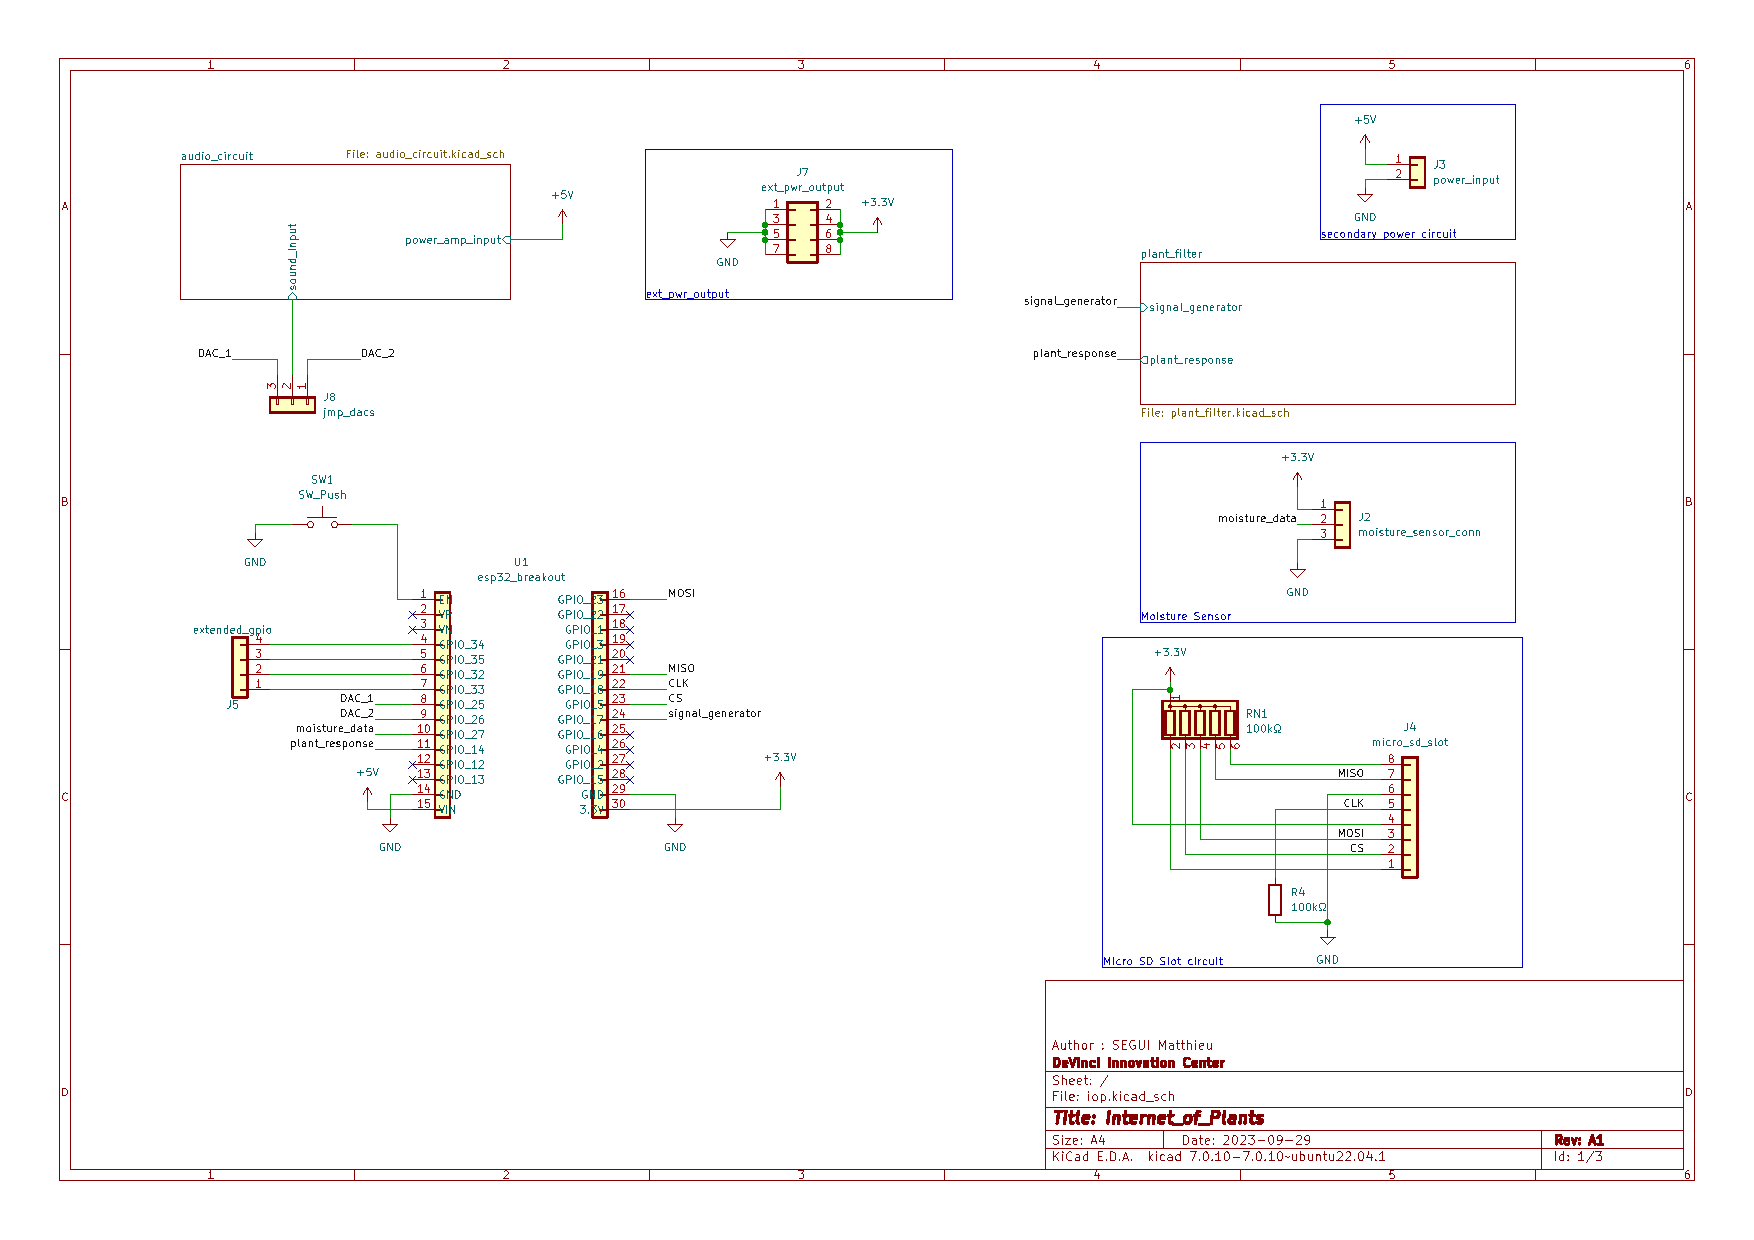
\includegraphics[width=\textwidth]{images/iop.pdf}
    \caption{The core of the circuit, the microcontroller, an ESP32 Wroom 32. All the other parts of
    circuits are plugged in.} 
    \vspace{0.1cm}
    \label{fig:iop_schematic_main}
\end{figure}

The circuit component that allows us to read data from the plant is the electronic filter.
This filter has been designed by \textit{Jakub Nikonowicz} and \textit{Łukasz Matuszewski} 
from \textit{Politechnika Poznańska}.
Thanks to them, I adapted it for my application on my embedded device. 

\begin{figure}[h]
    \centering
    \includegraphics[width=\textwidth]{images/iop-plant_filter.pdf}
    \caption{The electronic circuit designed to capture the interaction by analyzing the electronic
    frequency response. The circuit includes 3 resistors, 3 inductors and 3 capacitors as main components} 
    \vspace{0.1cm}
    \label{fig:iop_schematic_filter}
\end{figure}

The last part of the circuit is the sound output/rendering. This circuit includes a small amplifier,
the LM386 from Texas Instruments. The rest of the circuit are components needed in order to 
induce amplification on the signal without creating to many noise and saturation.

\begin{figure}[h]
    \centering
    \includegraphics[width=\textwidth]{images/iop-audio_circuit.pdf}
    \caption{The sound output part of the circuit that is used to render the sound. 
    This part includes a small amplifier, the LM386. The circuit also includes the components necessary
    to control and handle the amplification (reduce noise and saturation)} 
    \vspace{0.1cm}
    \label{fig:iop_schematic_audio}
\end{figure}


Once the schematic is done, we have to route the tracks. It exists multiple way to route PCB 
(single-sided, double-sided, multiple layers). We choose double sided, 2 layers on each side of the PCB.

\begin{figure}[h]
    \centering
    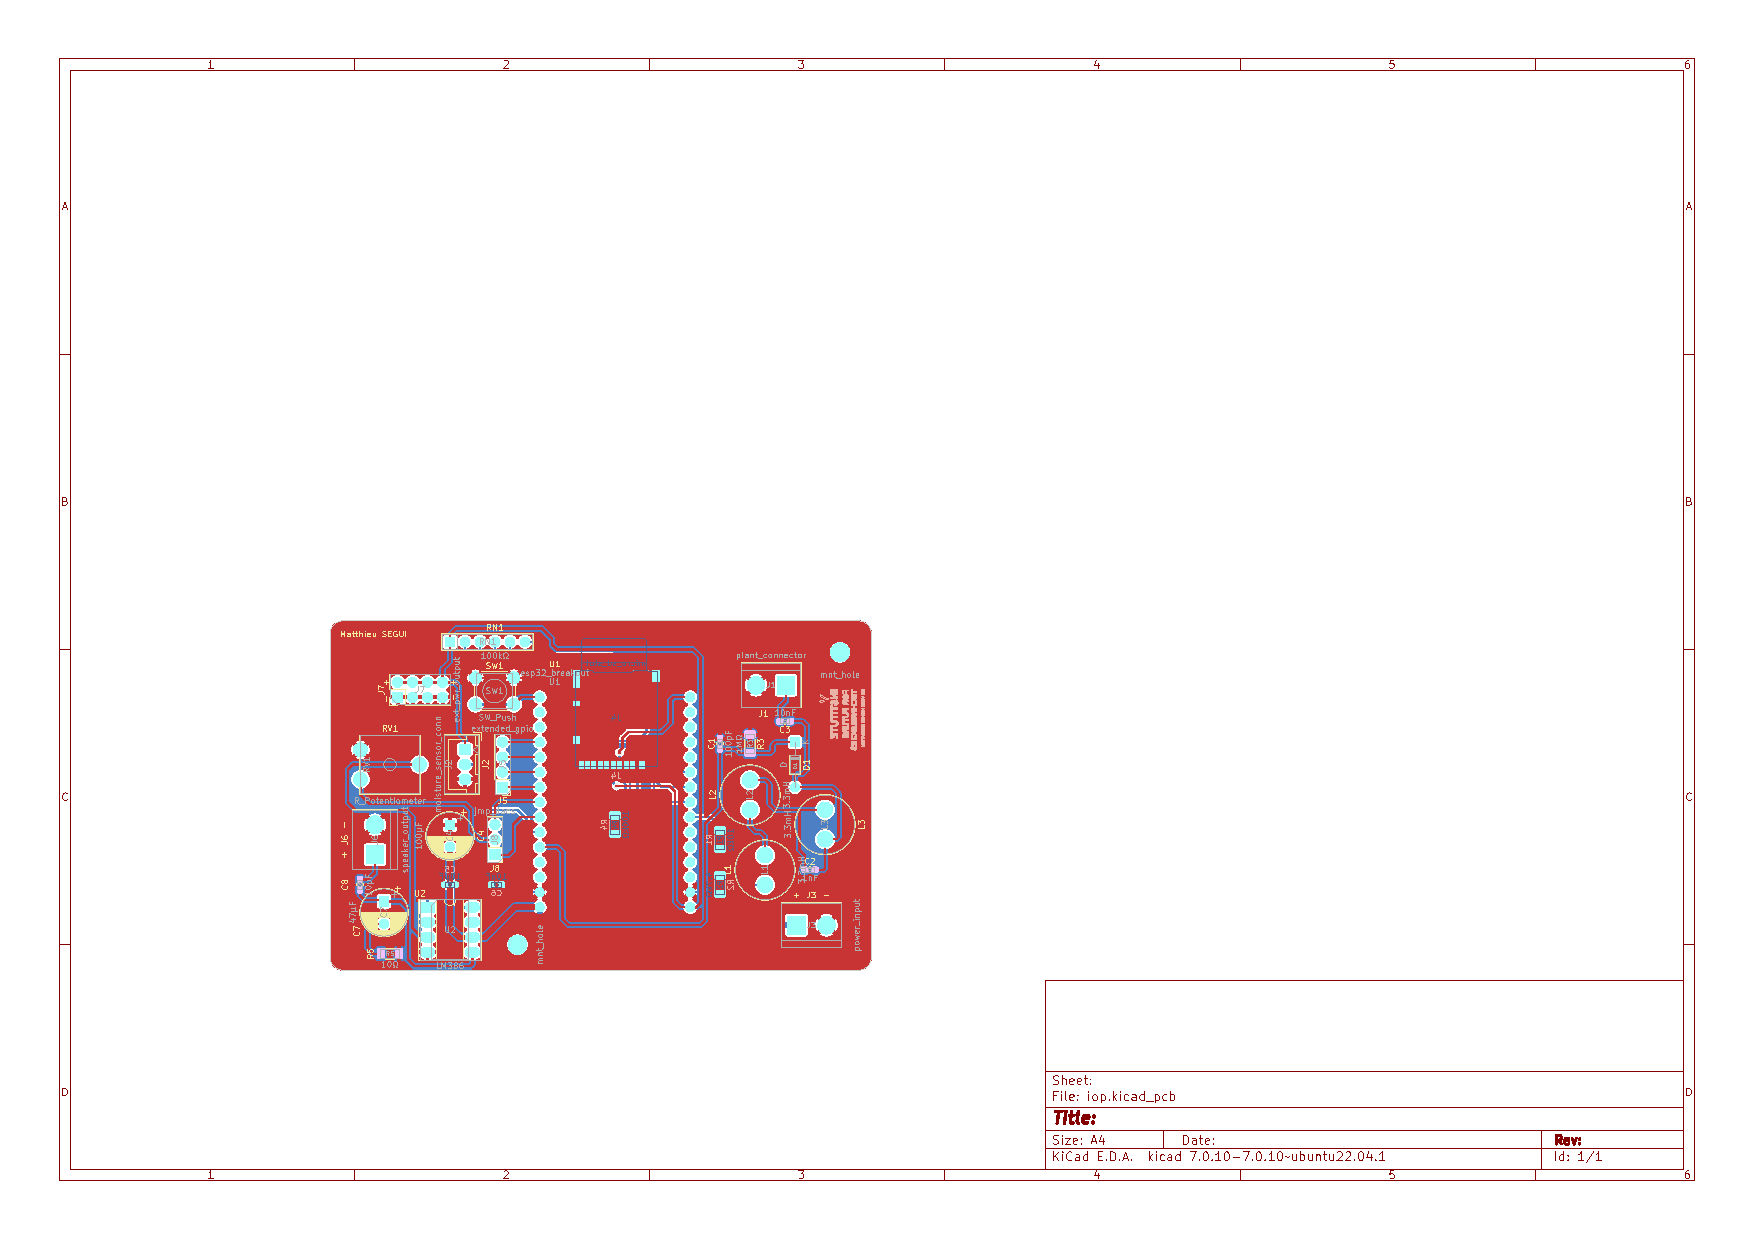
\includegraphics[width=\textwidth]{images/iop-routed_pcb.pdf}
    \caption{The routed double sided PCB.} 
    \vspace{0.1cm}
    \label{fig:iop_routed_pcb}
\end{figure}

Kicad also allows us to generated a 3D view of the future PCB.



\subsection{Human interaction}
\subsubsection{}
\subsubsection{User study}
\subsection{...}